% ---------------------------------------------------------------------
\chapter{Symmetry of Property Tensors}
\label{ch:symprop}


\section{Tensor quantities}

\begin{itemize}
\item {\bf Polar tensors} do not change sign when the handedness of the coordinate system changes
$$ a_{pqrs...} = T_{pi} T_{qj} T_{rk} T_{sl} ... a_{ijkl...}$$
\item {\bf Axial / Pseudo tensors} change sign when the handedness of the coordinate system changes
$$ a_{pqrs...} = \left| a \right| T_{pi} T_{qj} T_{rk} T_{sl} ... a_{ijkl...}$$
Here, $\left| a \right|$ is the determinant of the direction cosine matrix.
\end{itemize}

\section{Tensors that represent physical properties}

\begin{itemize}

\item
{\bf Constitutive relations} \index{Constitutive relation} are those that describe a physical phenomenon by connecting the cause with the effect through a material property.

In a constitutive relation, the entity that connects a tensor of order $m$ with a tensor of order $n$ is of the order $m+n$ by the quotient law of tensors. 

\item
{\bf Neumann's principle} \index{Neumann principle} : The symmetry group of any physical property of a crystal comprises the point symmetry group of the crystal.

A tensor that represents a physical property of a material should have at least the symmetry of the material.

\item
Pierre {\bf Curie symmetry principle} (1894) \index{Curie principle}: Effect is at least as symmetric as the cause. The symmetry of a crystal of known symmetry in the presence of external fields is given by the intersection of the symmetries of the crystal and the fields.

\end{itemize}


\begin{table}[h!]

\begin{tabular}[t]{lll}
{\bf Property} & {\bf Equation} &{\bf Quantities} \\

Pyroelectric effect & $\Delta P_i = \gamma_i \Delta T$ & \parbox[t]{18em}{electric polarisation, pyroelectric coefficient and change in temperature \\} \\

Thermal conduction & $ q_i = -k_{ij} \frac{dT}{dx_j}$ & \parbox[t]{18em}{heat flux, thermal conductivity and temperature gradient\\} \\

Electrical conduction & $ J_i = \sigma_{ij} E_j $ & \parbox[t]{18em}{electric current, electrical conductivity and electrical field\\} \\

Thermal expansion & $ e_{ij} = \alpha_{ij} \Delta T $ & \parbox[t]{18em}{thermal strain, thermal expansion coefficient and change in temperature\\} \\

Direct piezoelectric effect & $ P_i = d_{ijk} \sigma_{jk} $ & \parbox[t]{18em}{electric polarization, piezoelectric coefficient and stress tensor\\} \\

Inverse piezoelectric effect & $ e_{jk} = l_{ijk} E_i $ & \parbox[t]{18em}{strain, inverse piezoelectric coefficient and electric field\\} \\

Linear electrooptical effect & $ \Delta \eta_{ij} = r_{ijk} E_k $ & \parbox[t]{18em}{polarization constants, tensor of linear electrooptical effect and electric field\\} \\

Elasticity & $ e_{ij} = c_{ijkl} \sigma_{kl}$ & \parbox[t]{18em}{strain, elastic compliance and stress\\} 

\end{tabular}
\caption{Examples of common physical phenomena, adapted from \cite{perelomova}.}
\label{table:1}
\end{table}


Using the Neumann's principle, the tensor representing a property of a material should have the same symmetry as that of the material itself.

Liquids and glasses are isotropic ie., they have infinite symmetry \footnote{Only on a long range. They do have a short range order allegedly close to icosahedral in case of liquid metals}. The stuff remains the same in all the directions. So the physical property should also remain the same in all directions. So, the tensor representing the physical property of this stuff should be isotropic. That is, any arbitrary transformation of the co-ordinate system should leave the matrix containing the values of physical property unchanged. It is possible only if the property is representable by an isotropic tensor of corresponding order. Thus, for second order tensors such as thermal conductivity, diffusivity etc.,  of liquids only one value is necessary.

$$a_{ij} = a \delta_{ij}$$

Polycrystalline materials have crystals in all possible directions and as a bulk they behave as if the material is isotropic. Most of the engineering materials of interest are polycrystalline. Exceptions are highly textured materials (eg. after rolling) and single crystals (for turbine blades or semiconductor industry).

Take, for example, the second order tensor representing the thermal conductivity of a crystal. It should in general have 6 components (9 components become 6 thanks to the tensor being symmetric). Using the Curie principle, it can be shown as in section \ref{cubicsimplify} that for cubic crystals one needs to specify only one value for thermal conductivity.

% -----------------------------------------------------------------------

{\bf Examples of Tensor quantities}

\begin{tabular}{lll}
\hline \\
Order & Polar & Axial \\
\hline \\
0 & Specific heat & Rotary Power \\
1 & Pyroelectricity & Pyromagnetism \\
2 & Thermal expansion & Magnetoelectricity \\
3 & Piezoelectricity & Piezomagnetism \\
4 & Elastic compliance & Piezogyrotropy \\
\hline \\
\end{tabular}


% -----------------------------------------------------------------------
{\bf Quotient theorem}

\begin{itemize}
\item If $u_i$ and $v_j$ are tensors of order one and are related in every coordinate system as $u_i = b_{ij} v_j$ then $b_{ij}$ is a tensor of order two.

\item If $a_{ij}$ and $c_{ik}$ are tensors of order two and are related in every coordinate system as $a_{ij} b_{jk} = c_{ik}$ then $b_{jk}$ is a tensor of order two.

\item One can deduce the tensor character of most quantities that describe a physical process.

\item One can determine the highest possible rank of a tensor connecting a cause and effect in a constitutive equation.

\end{itemize}

% -----------------------------------------------------------------------

Tinder's book~\cite{tinder} has detailed analysis on how the tensor properties of crystals develop. An illustration of some common tensor quantities and their order is given in the figure~\ref{tensorexamples}. Newnham's book~\cite{newnham} also has a good discussion on the tensor properties of materials, their anisotropy, symmetry and structure.

\begin{figure}[h]
\begin{center}
\framebox{
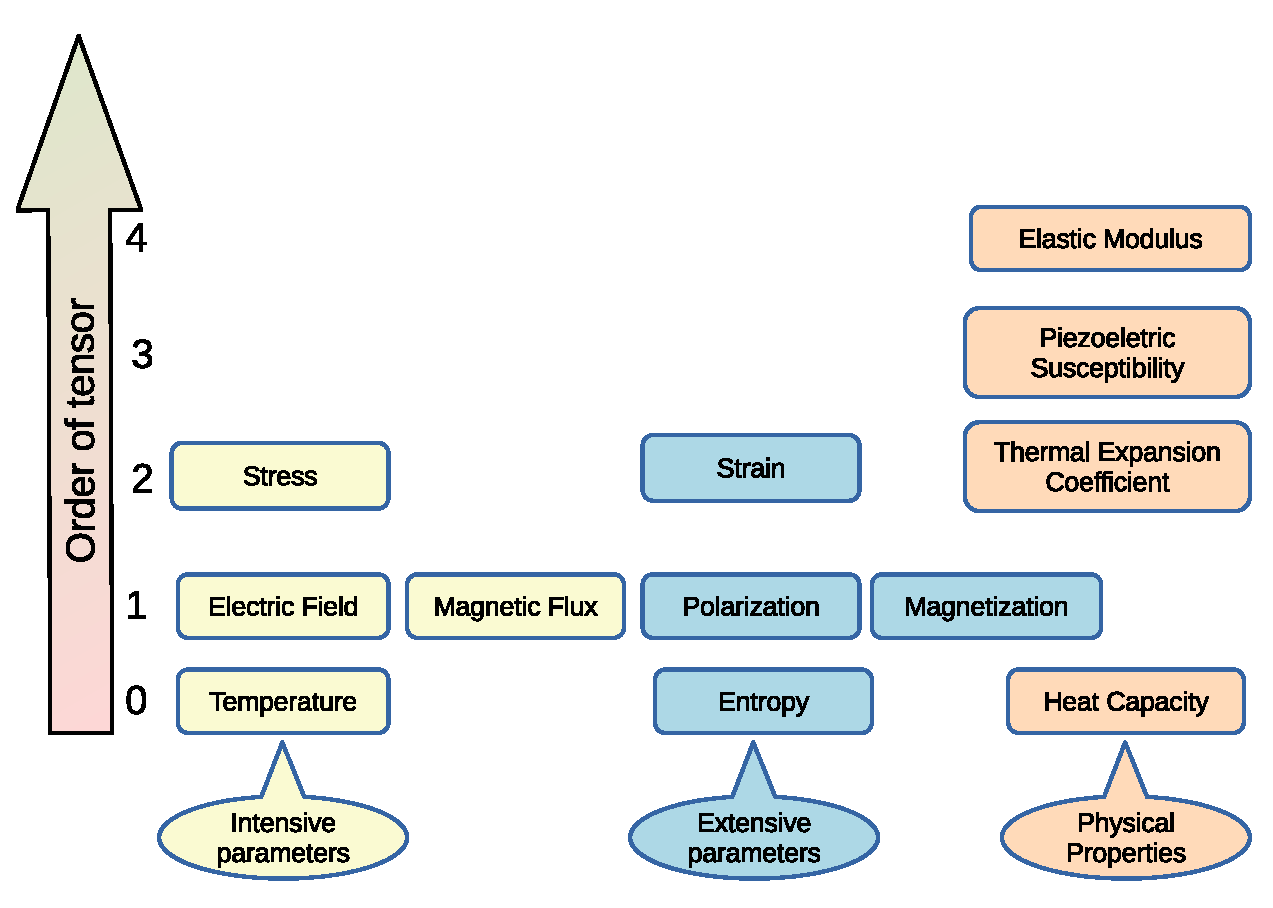
\includegraphics[scale=0.8]{images/c06-tensorexamples.eps}
 }
\end{center}
\caption{Examples of tensor quantities}
\label{tensorexamples}
\end{figure}

{\bf Constitutive relations}

{\bf Definition}
Constitutive relations are those that connect cause and effect.

$$ \text{Effect} = \text{Property} \, \times \, \text{Cause} $$

\begin{itemize}
\item Linear constitutive relations are quite popular.
\end{itemize}

% -----------------------------------------------------------------------

{\bf Heat conduction}

{\bf Fourier's law}
$$\vec{J} = -k \vec{\nabla}T$$

Thermal conductivity $k_{ij}$ is a tensor of order 2 since heat flux $\vec{J}$ and thermal gradient $\vec{\nabla} T$ are vectors.


% -----------------------------------------------------------------------

{\bf Elasticity}

{\bf Hooke's law}
$$ e = C \sigma $$

Compliance $C_{ijkl}$ is a tensor of order 4 since strain $e_{kl}$ and stress $\sigma_{ij}$ are tensors of order 2.


% -----------------------------------------------------------------------

{\bf Viscosity}

{\bf Newton's law}
$$ d_{ij} = \mu_{ijkl} {\partial u_k \over \partial x_l} $$

Viscosity $\mu_{ijkl}$ is a tensor of order 4 since strain rate ${\partial u_k \over \partial x_l}$ and deviatoric stress $d_{ij}$ are tensors of order 2.


% -----------------------------------------------------------------------

{\bf Thermal expansion}

$$ \sigma = \alpha \, \Delta T $$

Thermal expansion coefficient $\alpha_{ij}$ is a tensor of order 2 since stress $\sigma_{ij}$ is a tensor of order 2 and temperature difference $\Delta T$ is a scalar.


% -----------------------------------------------------------------------

{\bf Electrical resistance}

{\bf Ohm's law}
$$ \vec{E} = \rho \, \vec{J} $$

Electrical resistivity $\rho_{ij}$ is a tensor of order 2 since electric field strengh $\vec{E}$ and current density  $\vec{J}$ are vectors.


% -----------------------------------------------------------------------

{\bf Piezoelectric effect}

$$ P_i = d_{ijk} \sigma_{jk} $$

Direct piezeoelectric coefficient $d_{ijk}$ is a tensor of order 3 since polarization $\vec{P}$ is a vector and stress $\sigma_{jk}$ is a tensor of order 2.

Since centrosymmetric crystals cannot have properties of odd rank tensor, such crystals do not exhibit Piezeoelectricity.

% -----------------------------------------------------------------------

{\bf Electrostriction}

$$ x_{ij} = d_{ijk} E_k + M_{ijkl} E_k E_l $$

Direct piezeoelectric coefficient $d_{ijk}$ is a tensor of order 3 since polarization $\vec{P}$ is a vector and stress $\sigma_{jk}$ is a tensor of order 2.

Because of the second term, electrostriction is not limited to non-centrosymmetric crystals.


% -----------------------------------------------------------------------

{\bf Solute diffusion}

{\bf Fick's law}
$$ \vec{J}_A = -D \vec{\nabla} C_A $$

According to Fick's law, diffusion of a species A is down the concentration gradient. Actually it is down the chemical potential gradient. Since flux of species $\vec{J}_A$ and concentration (or chemical potential) gradient $\vec{\nabla} C_A$ (or $\vec{\nabla} \mu_A$) are vectors, diffusivity $D_{ij}$ must be a tensor of order 2.


% -----------------------------------------------------------------------


{\bf Curie Principle}


When certain causes lead to certain effects, the symmetry elements of the causes should be observed in these effects.


% -----------------------------------------------------------------------

{\bf Neumann Principle}

The symmetry of any physical property of a crystal must include the symmetry elements of the point group of the crystal.

% -----------------------------------------------------------------------

{\bf Symmetry effects on property tensors}

\begin{itemize}
\item Gases : Isotropic  
\item Liquids : Isotropic
\item Polycrystalline solids : Isotropic
\item Textured solids : Anisotropic, depending on type of texture
\item Single crystals : Anisotropic, depending on crystal symmetry
\end{itemize}

% -----------------------------------------------------------------------

% learning objective
\begin {lo3} [Tensors]
List number of independent components and the form of isotropic tensors
\end {lo3}

\section{Isotropic tensors}

\index{Tensor, isotropic}

{\bf Definition:} A tensor is isotropic if its elements donot change under {\em any} co-ordinate transformation\footnote{involving only rotations and reflections but not expansions or contractions ie., Det($T_{ij}$) is unity}.

\begin{itemize}

\item
Kronecker delta is an isotropic tensor of order two. The general form of an isotropic tensor of order two is 
$$ a_{ij} = a \delta_{ij}$$

\item
Levi-Civita density is an isotropic tensor of order three. Proof is given in section \ref{levicivitaisotropic} It is also referred to as alternating tensor or permutation tensor.

Relation between $\epsilon_{ijk}$ and $\delta_{ij}$ and the proof are given in equation \ref{epsilondelta}.

\item
$\delta_{ij}\delta_{kl}$ is an isotropic tensor of order four.

Most general form of an isotropic tensor of order four, where $\mu_1$, $\mu_2$ and $\mu_3$ are constants:

\begin{equation}
\boxed{\mu_{ijkl} = \mu_1\delta_{ij}\delta_{kl} + \mu_2\delta_{ik}\delta_{jl} + \mu_3\delta_{il}\delta_{jk}}
\end{equation} 

Proof is given in section \ref{isotensorfour}.

\end{itemize}


{\bf General forms of isotropic tensors for properties}

\begin{itemize}
\item Isotropic tensor of order 2 : $$\lambda \, \delta_{ij}$$
\item Isotropic tensor of order 3 : $$\lambda \, \epsilon_{ijk}$$
\item Isotropic tensor of order 4 : $$\lambda_1 \, \delta_{ij} \delta_{kl} + \lambda_2 \, \delta_{il} \delta_{kj} + \lambda_3 \, \delta_{ik} \delta_{jl}$$
\end{itemize}


% -----------------------------------------------------------------------

{\bf Imposing symmetry on property tensor}

If $a$ is a property tensor of order 2, use the following expression to identify the minimum number of elements of $a$ needed to represent it.
$$ a_{pq} = T_{pi} T_{qj} a_{ij} $$
Where $T_{pi}$ is the matrix corresponding to a coordinate transformation that represents a symmetry operation.

% -----------------------------------------------------------------------

\section{Symmetry elements of crystal classes}
Herrmann-Mauguin symbol is used for crystal class.


\begin{table}[h!]
\begin{tabular}{lll}
\hline \\
Crystal System & Crystal Class & Symmetry Elements \\
\hline \\
Monoclinic &  $2$ & $2 \parallel Z_2$ \\
Orthorhombic &  $222$ & $2 \parallel Z_1$ , $2 \parallel Z_2$ \\
Tetragonal & $\bar{4}2m$ & $\bar{4} \parallel Z_3$ , $2 \parallel Z_1$ \\
Hexagonal & $6/mmm$ & $6 \parallel Z_3$, $m \bot Z_3$, $m \bot Z_1$ \\
Cubic & $\bar{4}3m$ & $\bar{4} \parallel Z_3$, $3 \parallel [111]$ \\
\hline \\
\end{tabular}
\caption{Symmetry elements in some crystal systems}
\label{table:2}
\end{table}

% -----------------------------------------------------------------------

% learning objective
\begin {lo3} [Tensors]
Determine a transformation matrix suitable for a symmetry operation
\end {lo3}

{\bf Transformation matrices for symmetry operations}

Twofold rotation $2 \parallel Z_1$
\begin{equation*}
\left[
\begin{array}{lll}
1 & 0 & 0 \\
0 & -1 & 0 \\
0 & 0 & -1 \\
\end{array}
\right]
\end{equation*}

Mirror $m \bot Z_1$ 
\begin{equation*}
\left[
\begin{array}{lll}
-1 & 0 & 0 \\
0 & 1 & 0 \\
0 & 0 & 1 
\end{array}
\right]
\end{equation*}

Threefold rotation $3 \parallel Z_3$
\begin{equation*}
\left[
\begin{array}{lll}
-{1 \over 2} & {\sqrt{3} \over 2} & 0 \\
-{\sqrt{3} \over 2} & -{1 \over 2} & 0 \\
0 & 0 & 1 
\end{array}
\right]
\end{equation*}
Threefold rotation $3 \parallel [111]$
\begin{equation*}
\left[
\begin{array}{lll}
0 & 1 & 0 \\
0 & 0 & 1 \\
1 & 0 & 0 
\end{array}
\right]
\end{equation*}

Fourfold rotation $4 \parallel Z_3$
\begin{equation*}
\left[
\begin{array}{lll}
0 & 1 & 0 \\
-1 & 0 & 0 \\
0 & 0 & 1 
\end{array}
\right]
\end{equation*}

Fourfold inversion $\bar{4} \parallel Z_3$
\begin{equation*}
\left[
\begin{array}{lll}
0 & -1 & 0 \\
1 & 0 & 0 \\
0 & 0 & -1 
\end{array}
\right]
\end{equation*}


% -----------------------------------------------------------------------

{\bf Most property tensors are symmetric}

{\bf Microscopic Reversibility Principle}
For a system in thermodynamic equilibrium, every type of micromotion occurs just as often as its reverse.

{\bf Onsager's Reciprocity Principle}
Provided a proper choice is made for the fluxes and affinities, the matrix of phenomenological coefficients is symmetrical

As an implication of this, thermal conductivity $k_{ij}$ is a symmetric tensor.


% -----------------------------------------------------------------------
% learning objective
\begin {lo3} [Tensors]
Apply symmetry principles to reduce the number of independent components of a property tensor
\end {lo3}

\section{Scaffold to reduce components by symmetry operations}

\begin{mdframed}[style=tpscaffold1]
A crystal has a property $k_{ij}$ which is known to be a symmetric tensor of order 2. 

\begin{enumerate}
\item Write down the matrix representation of this tensor in its most general form.
\item If the crystal were to be rotated by 90 degrees, anti-clockwise about the $z$-axis, write down the new unit vectors in terms of the old unit vectors.
\item Looking at the above three relations, write down the transformation matrix $T$.
\item Determine the expression for the $k^*_{11}$ component of this tensor property in the new coordinate system.
\item Determine the expression for the $k^*_{21}$ component of this tensor property in the new coordinate system.
\item What does it mean to say $k^*_{11} = k_{11}$? or to say $k^*_{21} = k_{21}$?
\item If $k^*_{11} = k_{11}$, what can you infer?
\item If $k^*_{21} = k_{21}$, what can you infer?
\item If a four fold rotational symmetry is all that this crystal possesses, what can you say about the simplest form of $k$? Which crystal system would such a symmetry correspond to?
\item Extend the above steps for two other four fold rotations and arrive at the simplest possible form for $k$ for a cubic crystal.
\end{enumerate}
\end{mdframed}

{\bf Applying symmetry to property tensor}

Thermal conductivity $k_{ij}$, a second order symmetric tensor.
\begin{equation*}
k_{ij} = \left[
\begin{array}{lll}
k_{11} & k_{12} & k_{13} \\
k_{12} & k_{22} & k_{23} \\
k_{13} & k_{23} & k_{33}
\end{array}
\right]
\end{equation*}

Take the symmetry operation of 4 fold rotation (by $90^o$) about $\hat{x}_3$. Corresponding transformation matrix is:
\begin{equation*}
T = \left[
\begin{array}{lll}
0 & 1 & 0 \\
-1 & 0 & 0 \\
0 & 0 & 1
\end{array}
\right] 
\end{equation*}


Combining Neumann Principle and the definition of a second order tensor,
$$ k_{pq} = T_{pi} T_{qj} k_{ij} $$
\begin{enumerate}
\item Pick a combination of $p \, \& \, q$
\item Expand RHS, knowing not all terms of T are non-zero.
\item Repeat for all possible symmetry operations
\end{enumerate}


Using : $T_{12} = T_{33} = 1$, $T_{21}=-1$ and $ k_{pq} = T_{pi} T_{qj} k_{ij} $
$$k_{11} = T_{1i}T_{1j}k_{ij} = T_{12} T_{12} k_{22} = k_{22} \implies k_{11} = k_{22}$$

Similarly,
$$k_{21} = T_{2i} T_{1j} k_{ij} = T_{21} T_{12} k_{12} = -k_{12} = -k_{21} \implies k_{21} = k_{12} = 0$$

Using remaining symmetry operations, one can see that all off diagonal terms of $k_{ij}$ vanish and all diagonal terms are same.
\begin{equation*}
k_{ij} = \left[
\begin{array}{lll}
k_{11} & 0 & 0 \\
0 & k_{11} & 0 \\
0 & 0 & k_{11}
\end{array}
\right] = k_{11} \delta_{ij}
\end{equation*}


% -----------------------------------------------------------------------

\section{Components of a symmetric tensor property}

Triclinic:
\begin{equation*}
\left[
\begin{array}{lll}
S_{11} & S_{12} & S_{13} \\
 & S_{22} & S_{23} \\
 &  & S_{33} \\
\end{array}
\right]
\end{equation*}

Monoclinic:
\begin{equation*}
\left[
\begin{array}{lll}
S_{11} & 0 & S_{13} \\
 & S_{22} & 0 \\
 &  & S_{33} \\
\end{array}
\right]
\end{equation*}

Orthorhombic:
\begin{equation*}
\left[
\begin{array}{lll}
S_{11} & 0 & 0 \\
 & S_{22} & 0 \\
 &  & S_{33} \\
\end{array}
\right]
\end{equation*}

Tetragonal, trigonal, hexagonal:
\begin{equation*}
\left[
\begin{array}{lll}
S_{11} & 0 & 0 \\
 & S_{11} & 0 \\
 &  & S_{33} \\
\end{array}
\right]
\end{equation*}

Cubic:
\begin{equation*}
\left[
\begin{array}{lll}
S_{11} & 0 & 0 \\
 & S_{11} & 0 \\
 &  & S_{11} \\
\end{array}
\right]
\end{equation*}

% -----------------------------------------------------------------------

{\bf Diagonalizability theorem}

\begin{itemize}

\item There exists a coordinate system in which a symmetric tensor can be represented only by diagonal elements.
\item Stress is a symmetric tensor because of continuum approximation.
\item This is used to arrive at the principal components of a stress state.
\end{itemize}

% ---------------------------------------------------------------------

\section{Summary}

\begin{enumerate}
\item Kronecker delta $\delta_{ij}$ can be used: to simplify subscripts, $a_{ik} \delta_{ij} = a_{jk}$, to represent inner / dot products and to represent an isotropic tensor of order two.
\item Levi-Civita / permutation matrix can be used: to represent cross products, to arrive at determinants of matrices and to represent an isotropic tensor of order three.
\item Kronecker delta and Levi-Civita symbol are connected as: $\epsilon_{ijk} \epsilon_{klm} = \delta_{il} \delta_{jm} - \delta_{im} \delta_{jl}$ and $\epsilon_{ijk} \epsilon_{ijm} = 2 \delta_{km}$.
\end{enumerate}

% ---------------------------------------------------------------------
